In this chapter, we delve into the experimentation with Flamingo for zero-shot image captioning. We designed our study to evaluate Flamingo's capacity to generate accurate and contextually rich captions without prior training on specific image datasets. This approach is particularly challenging and promising, as it relies solely on the model's pre-existing knowledge and its ability to generalize from it.

\section{Prompting Flamingo for zero-shot image captioning}

To conduct a comprehensive evaluation, we employed three different prompts, as outlined in Table \ref{tab:cap-prompts}. 

\begin{table}[h]
    \centering
    \begin{tabular}{cl}
        \rowcolor{lightgreen} \textbf{Index} & \textbf{Prompt} \\
        \rowcolor{lightgreen} 0 & “An image of” \\
        \rowcolor{lightgreen} 1 & “A complete caption for this image is:” \\
        \rowcolor{lightgreen} 2 & “Question: What can you say about the location and time of this image? Answer:”
    \end{tabular}
    \caption{Prompt variations for captioning using Flamingo.}
    \label{tab:cap-prompts}
\end{table}

Each prompt was carefully crafted to analyse various aspects of Flamingo's captioning abilities:

\begin{itemize}
    \item \textit{An image of:} This prompt is straightforward and open-ended, designed to assess the model's basic descriptive capabilities. It serves as a baseline to understand how Flamingo interprets and narrates the visual content without specific guidance.
    \item \textit{A complete caption for this image is:}: With this prompt, we aim to direct the model to produce a more detailed and structured response. It's an attempt to encourage Flamingo to not only describe what's visible, but also to infer and articulate a more comprehensive understanding of the image.
    \item \textit{Question: What can you say about the location and time of this image? Answer:}: This prompt is particularly aimed at evaluating Flamingo's ability to contextualize the image. By asking for the location and time, we are testing the model's capacity to deduce historical and geographical information, which often requires a higher level of inference and understanding.

\end{itemize}



We aim to evaluate the predicted captions based on distinctiveness, coherence, fluency, relevance, and completeness. Additionally, we are interested in the model's ability to contextualize an image in terms of time and place.

% \section{Results}


\section{Discussion \& Conclusions}

We perform a qualitative analysis of the results by sampling five images per class and evaluating Flamingo's captioning abilities based on various aspects, inspired by the \cite{fu2023mme} evaluation benchmarks. The generated captions for all prompts are displayed on the table accessible at \url{https://github.com/dh-epfl-students/dhlab-image-captioning/blob/main/FLAMINGO/cap_summary.html}. 

\subsubsection{Qualitative analysis}


The predictions are generally distinctive. Moreover, it generally recognizes the regions of the world on a map, in a picture with hints such as country flags or signs that require OCR. The generated text for a few maps illustrate this point and can be observed in Table \ref{tab:distinctiveness}.

\begin{table}[h]
    \centering
    \begin{tabular}{c|c|c}
    \setlength{\tabcolsep}{5pt}
        \textbf{Image} & \textbf{Caption} & \textbf{Analysis}\\
        \hline
        \begin{minipage}[c]{4cm}
            \includegraphics[width=\linewidth]{Images/map1.png}
        \end{minipage} & 
        \begin{minipage}[c]{0.3\linewidth}
            “a map of the Middle East during the First World War.”
        \end{minipage} & 
        \begin{minipage}[c]{0.3\linewidth}
            This is indeed a map of the Middle East. However, it is after WWI since Transjordan which appears at the bottom was only founded in 1921.
        \end{minipage} \\
        \hline
        \begin{minipage}[c]{4cm}
            \includegraphics[width=\linewidth]{Images/map5.png}
        \end{minipage} & 
        \begin{minipage}[c]{0.3\linewidth}
            “the Ordnance Survey One-inch to the mile map of the Lake District, c.18”
        \end{minipage} &
        \begin{minipage}[c]{0.3\linewidth}
            The caption is false since this is a map of the surroundings of Salgesch in Switzerland.
        \end{minipage} \\
        \hline
        \begin{minipage}[c]{4cm}
            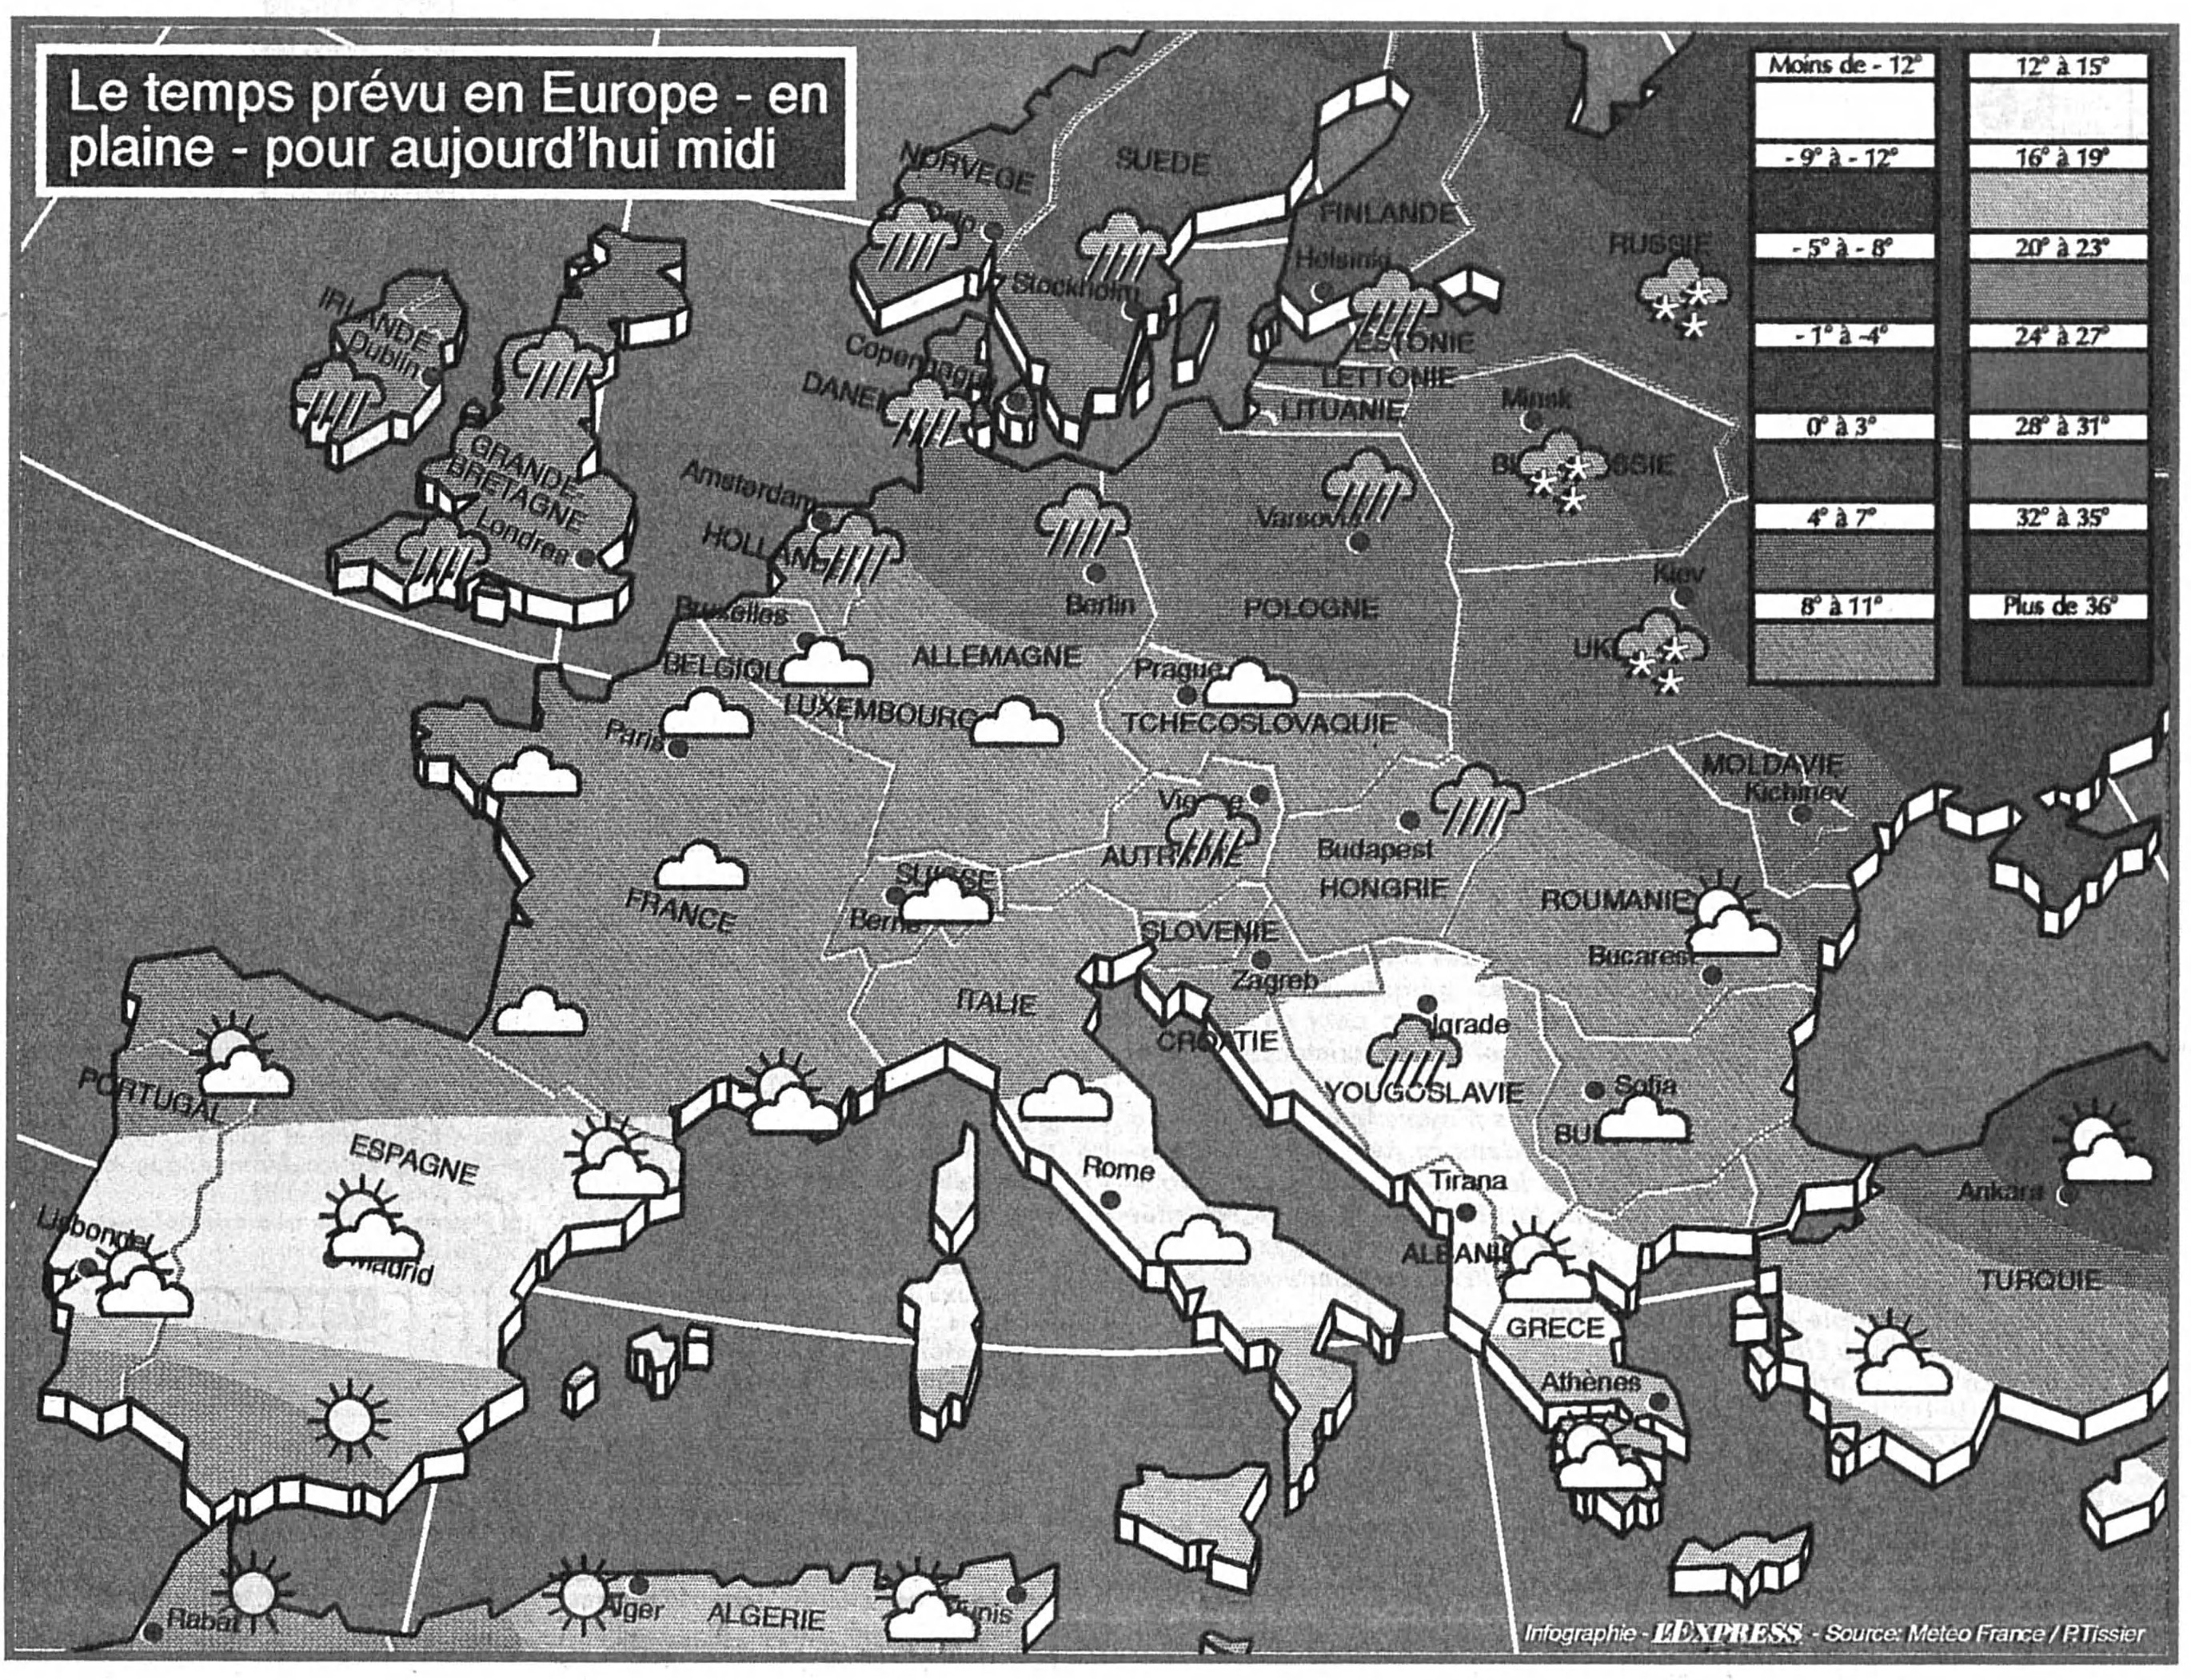
\includegraphics[width=\linewidth]{Images/map3.png}
        \end{minipage} & 
        \begin{minipage}[c]{0.3\linewidth}
            "a map of the European continent showing the weather conditions for the month of May."
        \end{minipage} & 
        \begin{minipage}[c]{0.3\linewidth}
           The caption appears accurate, inferring May from weather conditions, despite the absence of an explicit OCR indication.
        \end{minipage} \\
        \hline
        \begin{minipage}[c]{4cm}
            \includegraphics[width=\linewidth]{Images/map4.png}
        \end{minipage} & 
        \begin{minipage}[c]{0.3\linewidth}
            "a map of the Soviet Union and its allies in the Second World War."
        \end{minipage} &
        \begin{minipage}[c]{0.3\linewidth}
            The map indeed includes a part of URSS, Canada and the USA, which were all allies in WWII. However, it also includes Japan, and the caption seems to miss what is happening in Hawaii.
        \end{minipage} \\
    \end{tabular}
    \caption{Examples of generated captions for the prompt \textit{"An image of"} on maps.}
    \label{tab:distinctiveness}
\end{table}
\clearpage

As for the timing, it is sometimes capable of accurately situating the image in the correct time period, but at other times, it makes false assumptions. As seen in Table \ref{tab:temporal-context}, it recognizes that the dress is indeed from the 1920s, and that the \textit{Special mode} logo is from 1970.

\begin{table}[ht]
    \centering
    \setlength{\tabcolsep}{5pt}  % Adjust the separation between columns
    \begin{tabular}{c|c|c|c}
        \textbf{Image} & \textbf{Caption} & \textbf{Image} & \textbf{Caption} \\
        \hline
        \begin{minipage}[c]{0.2\linewidth}
            \includegraphics[width=\linewidth]{Images/dress.png}
        \end{minipage} &
        \begin{minipage}[c]{0.2\linewidth}
            Question: What can you say about the location and time of this image? Answer: It was taken in the 1920s.
        \end{minipage} &
        \begin{minipage}[c]{0.2\linewidth}
            \includegraphics[width=\linewidth]{Images/special.png}
        \end{minipage} &
        \begin{minipage}[c]{0.3\linewidth}
            Question: What can you say about the location and time of this image? Answer: It was taken in Paris, France, in the early 1970s.
        \end{minipage} \\
    \end{tabular}
    \caption{Examples of correct temporal contextualization}
    \label{tab:temporal-context}
\end{table}

However, the model is frequently incoherent. In fact, for the same image but different captions, it can generate contradictory information. This is illustrated using the captions of a map of Salgesch, Switzerland, in Table \ref{tab:coherence}.

\begin{table}[ht]
    \centering
    \setlength{\tabcolsep}{5pt}  % Adjust the separation between columns
    \begin{tabular}{c|c|c|c}
        \textbf{Image} & \textbf{Caption 1} & \textbf{Caption 2} & \textbf{Caption 3} \\
        \hline
        \begin{minipage}[c]{0.2\linewidth}
            \includegraphics[width=\linewidth]{Images/map5.png}
        \end{minipage} &
        \begin{minipage}[c]{0.2\linewidth}
            A complete caption for this image is: Aerial view of the summit of Mount
        \end{minipage} &
        \begin{minipage}[c]{0.2\linewidth}
            the Ordnance Survey One-inch to the mile map of the Lake District, c.18
        \end{minipage} &
        \begin{minipage}[c]{0.3\linewidth}
            Question: What can you say about the location and time of this image? Answer: This is a map of the location of the Battle of the Little Bighorn in 1876.
        \end{minipage} \\
    \end{tabular}
    \caption{Example of an incoherency.}
    \label{tab:coherence}
\end{table}

Furthermore, for a few images that take place in a general context, Flamingo tends to generate very specific captions. Our hypothesis from the sample observed is that if it recognizes a few elements that coincide with an image it was trained on, the model associates it to the paired caption it was trained on. Examples are shown in Table \ref{tab:out-of-context}. It seems that the model lacks the ability to analyse correctly the context in a picture. Rather, it tries to find similarities between the training data and the given picture, then outputs the caption it was trained on.

\begin{table}[ht]
    \centering
    \setlength{\tabcolsep}{5pt}  % Adjust the separation between columns
    \begin{tabular}{c|c|c|c}
        \textbf{Image} & \textbf{Caption} & \textbf{Image} & \textbf{Caption} \\
        \hline
        \begin{minipage}[c]{0.2\linewidth}
            \includegraphics[width=\linewidth]{Images/graph1.png}
        \end{minipage} &
        \begin{minipage}[c]{0.2\linewidth}
            An image of: Table 1 from the report of the Commission of Enquiry into the Condition of the Indian Population in [...]
        \end{minipage} &
        \begin{minipage}[c]{0.2\linewidth}
            \includegraphics[width=\linewidth]{Images/building.png}
        \end{minipage} &
        \begin{minipage}[c]{0.3\linewidth}
            A complete caption for this image is: The old school house, built in 1856, is now the home of the Historical Society.
        \end{minipage} \\
    \end{tabular}
    \caption{Example of Flamingo assuming a context based on its training data.}
    \label{tab:out-of-context}
\end{table}









